\clearpage
\setcounter{page}{1}
\maketitlesupplementary
\section{Implementation Details} 

We conduct training for 20k iterations and set \( N_{\mathrm{iter}}=10k\) for both datasets. Feature Adaptive Densification and Prune is applied at 10k iterations and patch-based density controlling strategy at 8k iterations for stability. Further more, we set \( \lambda_{\text{low}} = 2.0 \) and \( \lambda_{\text{high}} = 0.8 \). In addition, the parameter $\tau_{\text{sparse}}$ is set to be the number of Gaussians in the top 90$\%$ of patches sorted by point density in descending order, while $\tau_{\text{high}}$ to be the number of top 10$\%$. Besides, the number of generated views is set to 4×, meaning that 3 generated views are inserted between every two training views. Frame interpolation is introduced after 2k iterations, with its loss evaluated at an interval of every 10 iterations. Starting from iteration 2000, it is applied for the first 100 iterations of every subsequent 200-iteration cycle, and disabled for the remaining 100 iterations. We first set $\lambda_{g}=0.075$, which increases as the training iterations grows. SAUGE~\cite{liufu2025sauge}, a model based on SAM, is used to extract the edge of each training image. The co-pruning parameters are set following the configuration used in CoR-GS~\cite{zhang2024cor}. HeroGS is initialized with point clouds and precomputed camera poses from COLMAP.

\textbf{Selection Module.}
The Gaussian fields are first trained for 2000 iterations without image-level guidance.
After this stage, pseudo-label images are filtered based on their quality, and the high-quality ones are used for subsequent supervision. 
The selection metric is computed as:
\begin{equation}
M = \lambda_1 \| I^{\alpha} - \hat{I}^{\alpha} \| + \lambda_2 \mathcal{L}_{D\text{-}SSIM} \, \mathrm{Cor}(\hat{I}^{\alpha}, I^{\alpha}),
\end{equation}
where $I^{\alpha}$ denotes a pseudo-label, and $\hat{I}^{\alpha}$ represents the corresponding rendered image. 
To avoid the influence of model instability during the early training phase, we progressively re-evaluate and re-select pseudo-labels according to the rendered outputs as training proceeds.
If there are $N$ pseudo-labeled images in total, $N/2$ images with the smallest values of $M$ (i.e., those closest to the rendered results) are selected as high-quality supervision for the subsequent training phase.

\begin{figure}[h]
  \centering
  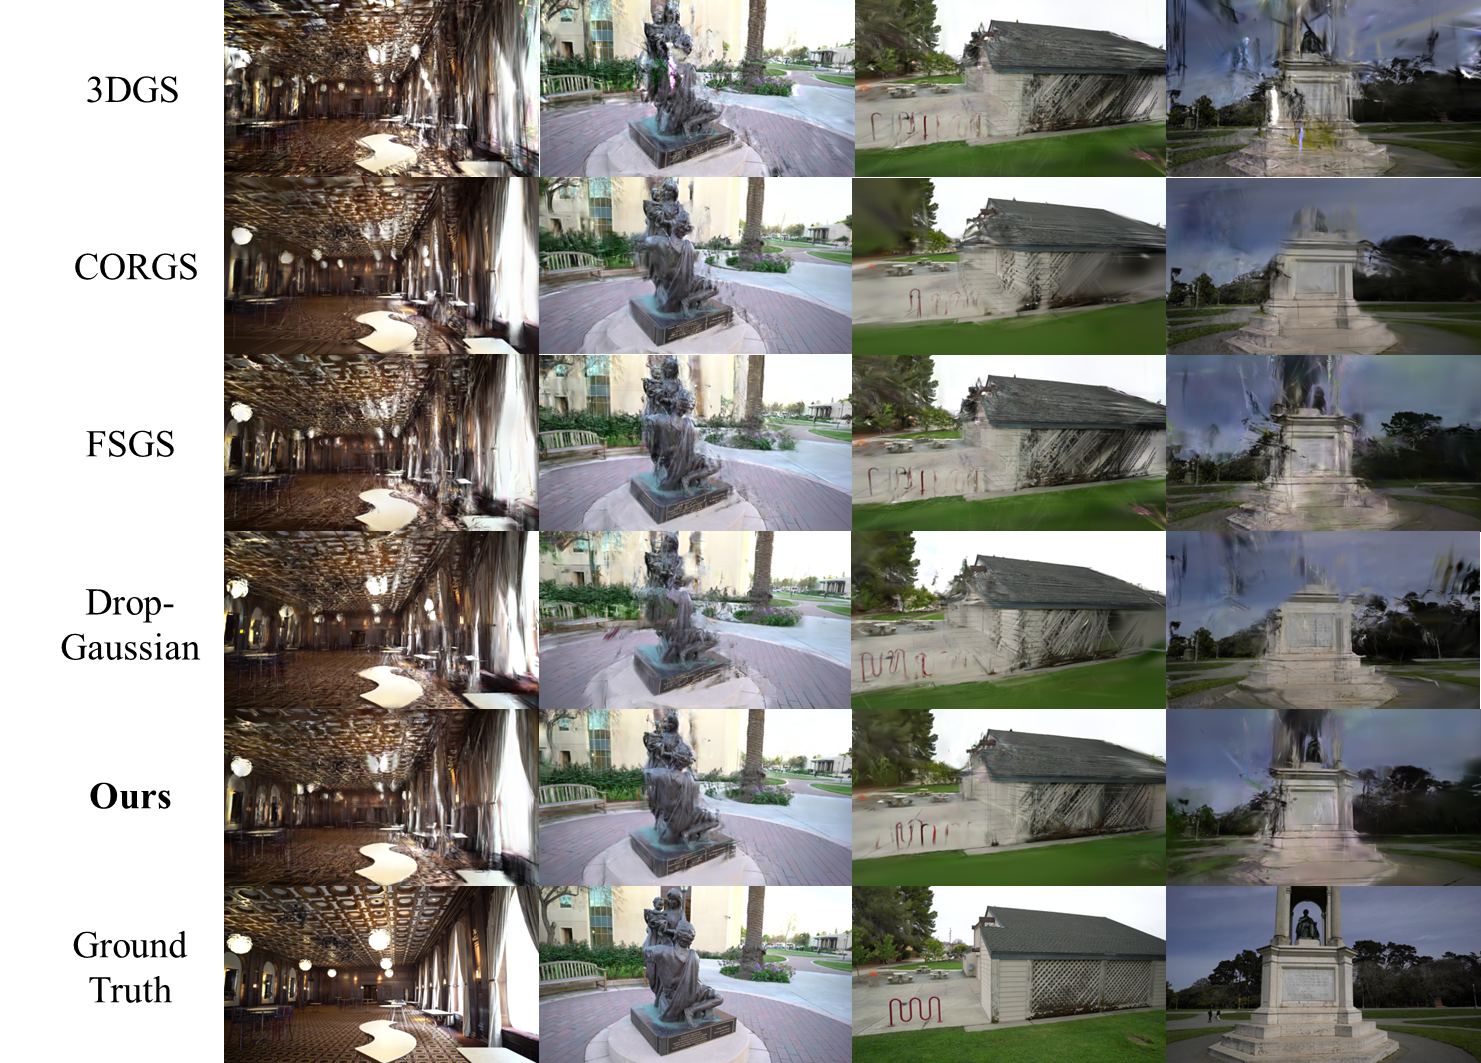
\includegraphics[width=0.95\columnwidth]{imgs/T_T_visualize.png}
%   \vspace{-5pt}
  \caption{\textbf{Qualitative Comparison on Tanks for 3 training views.} In large-scale dataset, 3DGS and DropGaussian struggles to maintain geometry and texture fidelity, exhibiting significant artifacts. FSGS and CoR-GS recover coarse structure yet still exhibit over-smoothed geometry and artifacts. In contrast, HeroGS reconstruct fine structures and high-frequency textures.
  }
%   \vspace{-5pt}
  \label{fig:T_T_vis}
\end{figure}

\section{More Comparison Results}
\begin{table}[t]
\centering
\renewcommand{\arraystretch}{1.1}
\setlength{\tabcolsep}{1pt}

  \begin{tabularx}{\columnwidth}{l|*{6}{Y}}

  \hline
  \multirow{2}{*}{Methods} & \multicolumn{3}{c}{12 views} & \multicolumn{3}{c}{24 views} \\
  & PSNR↑ & SSIM↑ & LPIPS↓ & PSNR↑ & SSIM↑ & LPIPS↓\\
  \hline
  3DGS      & 18.44 & 0.521 & 0.385 & 23.22 & 0.730 & 0.234\\
  FSGS      & 18.93 & 0.539 & 0.380 & 23.46 & 0.738 & 0.237\\
  CoR-GS      & \underline{19.59} & \underline{0.578} & 0.374 & 23.39 & 0.727 & 0.272\\
  DropGaussian      & 19.49 & 0.573 & \textbf{0.366} & \underline{24.03} & \underline{0.762} & \textbf{0.225}\\
  HeroGS      & \textbf{19.99} & \textbf{0.591} & \underline{0.373} & \textbf{24.18} & \textbf{0.766} & \underline{0.229}\\
  \hline

  \end{tabularx}\
  \caption{\textbf{Quantitative results on Mip-NeRF360~\cite{Barron_2022_CVPR} with 12, 24 training views.} }
  \label{tab:QUA_Mip}
\end{table}

\begin{figure*}[h]
  \centering
  \includegraphics[width=0.85\textwidth]{imgs/Fig8_HeroGS.pdf}
%   \vspace{-5pt}
  \caption{\textbf{ Ablation study on LLFF dataset showing the impact of varying interpolation factor $S$ on PSNR, SSIM, and LPIPS.}
  }
  \label{fig:Inter_factor}
\end{figure*}
%   \vspace{-5pt}

\textbf{Ablation on Selection Module.}
Table~\ref{tab:Ablation_selection} demonstrates that incorporating the Selection module yields consistent improvements across all evaluation metrics, this improvement verifies the effectiveness of filtering out low-quality pseudo-labels, which stabilizes supervision and prevents the propagation of noise during optimization. In essence, the Selection module ensures that only reliable pseudo-labels contribute to training, leading to cleaner gradients and more robust convergence under sparse-view settings.
\begin{table}[t]
\centering

%\resizebox{.95\columnwidth}{!}{
  \begin{tabularx}{0.5\textwidth}{l|*{3}{Y}}

  \hline
  Settings & PSNR & SSIM & LPIPS\\
  \hline
  w/o Selection      & 21.19 & 0.736 &  0.190\\
  All     & \textbf{21.30} & \textbf{0.739} & \textbf{0.189}\\
  \hline
  
  \end{tabularx}
  \caption{Ablation study on Selection module on LLFF dataset for 3 training views. }
  \label{tab:Ablation_selection}
\end{table}





\begin{figure*}[t]
  \centering
  \includegraphics[width=0.91\textwidth]{imgs/Fig9_HeroGS.pdf}
%   \vspace{-7pt}
  \caption{
  \textbf{Qualitative comparison of depth rendering quality.}
  We visualize the depth maps rendered from the reconstructed 3D Gaussian fields of different methods and our proposed HeroGS framework. 
  The visualizations show that our method produces more consistent and artifact-free depth results with finer geometry structure preservation. 
  }


%   \vspace{-11pt}
  \label{fig:depth_vis}
\end{figure*}

\textbf{Depth Visualization.}
Fig.~\ref{fig:depth_vis} presents qualitative comparisons of depth maps rendered from Gaussian fields reconstructed by 3DGS, DRGS, FSGS, and our proposed HeroGS framework. 3DGS suffers from severe artifacts and structural inconsistencies, particularly near object boundaries and occlusions. DRGS improves upon this with depth supervision, yet still exhibits oversmoothing and background bleeding, compromising geometric fidelity.

FSGS enhances robustness via Proximity-guided Gaussian Unpooling, capturing global shapes more reliably but still fails to preserve finer geometric details, leading to blurry depth transitions. In contrast, HeroGS framework yields significantly sharper and cleaner depth maps. It better preserves thin structures—such as plant stems and insect limbs—and maintains clear depth discontinuities. The consistent performance gains can be ascribed to the multi-level hierarchical guidance and the synergistic coupling across different supervision levels, which jointly refine Gaussian distributions for more robust reconstruction.

\textbf{Mip-NeRF360.}
To further demonstrate the generalizability of HeroGS in unbounded real-world scenes, it is evaluated on the Mip-NeRF360 dataset using 12 and 24 input views with resolutions downsampled by 8$\times$. As shown in Tab.~\ref{tab:QUA_Mip}, HeroGS consistently achieves the best performance across all metrics. In particular, it surpasses the second-best method by a notable margin of +0.5 dB in PSNR and +0.02 in SSIM on average, while maintaining competitive perceptual quality in terms of LPIPS. These results highlight that HeroGS can effectively handle complex illumination and large-scale geometry, showing superior robustness under sparse-input conditions and strong generalization to unbounded scene reconstruction.

\section{Discussion}
\textbf{Another View of the Overall Framework.}
In our framework, a dense set of RGB images is synthesized as pseudo-labels, which, together with the training views, jointly constrain the optimization of the Gaussian Splatting field. To mitigate the potential 3D geometric inconsistencies introduced by the primary pseudo-labels, we design a refinement pipeline that incorporates two synergistic submodules. First, the Feature-Adaptive Densification and Pruning (FADP) enhances features discriminability using training views through adaptive densification controlling, while stochastically pruning redundant textures to prevent overfitting to label noise. This process encourages finer representation of geometry and textures in high-frequency regions. Second, the Co-Pruned Geometry Consistency (CPG) adopts a freeze-and-co-prune strategy to suppress erroneous structures arising from pseudo-label supervision, thereby mitigating distortion artifacts and improving global consistency. Pseudo-labels generation and two refinement submodules form a coherent framework that not only enhances supervision quality but also preserves structural fidelity under sparse-view conditions.

\textbf{Limitation and Future Work.}
Although our framework forms a hierarchical guidance across multiple levels, the current implementation only applies the Feature-Adaptive Densification and Pruning (FADP) once during the training phase. 
This design is motivated by the observation that a single round of FADP is sufficient to recover most high-frequency geometric details, whereas additional iterations only bring marginal gains in performance.
In future work, we plan to extend this mechanism into a multi-stage adaptive refinement process, where density control can be repeatedly guided by the pseudo-labels from the image level. 
Such a recurrent optimization loop would enable dynamic feedback across levels, thereby further enhancing geometric precision and strengthening global consistency in sparse-view reconstruction tasks.